\documentclass{article}
\usepackage{tikz}
\usepackage{amsmath} % Para usar \text en matemáticas

\begin{document}
	
	\begin{center}
		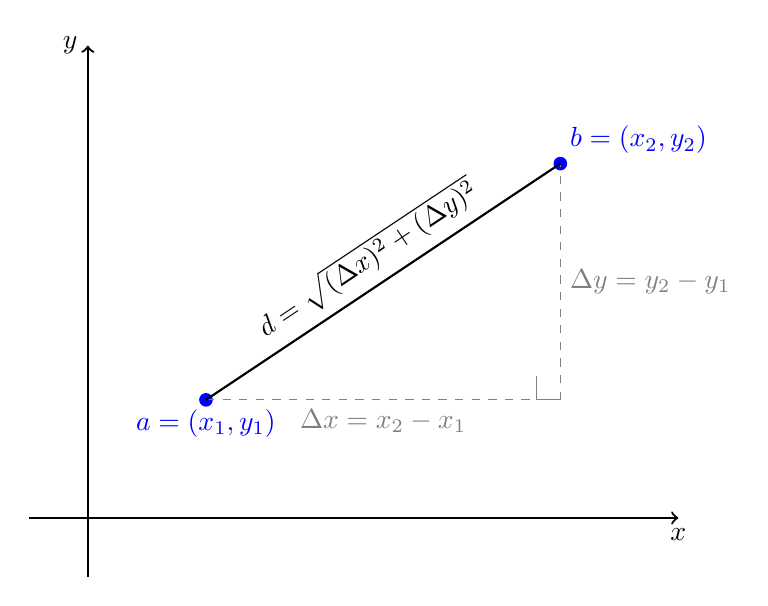
\begin{tikzpicture}[scale=1.5]
			
			% Ejes
			\draw[thick,->] (-0.5,0) -- (5,0) node[below] {$x$}; % Eje x
			\draw[thick,->] (0,-0.5) -- (0,4) node[left] {$y$};  % Eje y
			
			% Definir los puntos
			\coordinate (a) at (1,1);       % Punto a
			\coordinate (b) at (4,3);       % Punto b
			
			% Dibujar los puntos
			\filldraw[blue] (a) circle (1.5pt) node[below] {$a = (x_1, y_1)$};
			\filldraw[blue] (b) circle (1.5pt) node[above right] {$b = (x_2, y_2)$};
			
			% Dibujar las líneas de diferencia en las coordenadas
			\draw[dashed, gray] (a) -- (b |- a) node[midway, below] {$\Delta x = x_2 - x_1$}; % Línea horizontal
			\draw[dashed, gray] (b |- a) -- (b) node[midway, right] {$\Delta y = y_2 - y_1$};  % Línea vertical
			
			% Dibujar la hipotenusa (distancia entre a y b) en negro
			\draw[thick, black] (a) -- (b) node[midway, above, sloped] {$d = \sqrt{(\Delta x)^2 + (\Delta y)^2}$};
			
			% Ángulo recto
			\draw[gray] (b |- a) -- ++(-0.2,0) -- ++(0,0.2);
			
		\end{tikzpicture}
	\end{center}
	
\end{document}